% Golden Spiral can be approximated with Golden ratio or Fibonacci sequence.
% Golden Ratio: a+b/a = a/b

\documentclass{beamer}
\usepackage[utf8]{inputenc}
\usepackage[T1]{fontenc}

\usetheme{Cuerna}
\usecolortheme{default}
% default, bluesimplex, lettuce, brick

\title{TITLE}
\author{Shayan Amani}

\date{DATE 2018}
\institute{Department of Computer Science, University of New Hampshire}

\begin{document}

  \begin{frame}
    \titlepage
  \end{frame}

  \begin{frame}
    \frametitle{Pneumonoultramicroscopicsilicovolcanoconiosis}
    \framesubtitle{SUB}

  \end{frame}


    \section{Questions}
\begin{itemize}
    \item 2000 samples for 10 times of 200 years. What kind of times?
    \item What are states? How many?
\end{itemize}

\section{Definition}
We have 2000 samples for 200 years. In terms of games, this is like a already played game and we have the history of the gameplay.

\subsection{State}
each row

\subsection{Action}
2 actions: 0 and 10.
$\epsilon$-greedy exploration is not applied, because we have no control over agent.

\subsection{Reward}
A summation according to it's definition.


\section{Methodology}
We can use either On-Policy or Off-Policy methods. From the given samples it could be simply inferred that a model-free algorithm is needed and the reason is that the problem doesn't provide the transition probabilities.


	%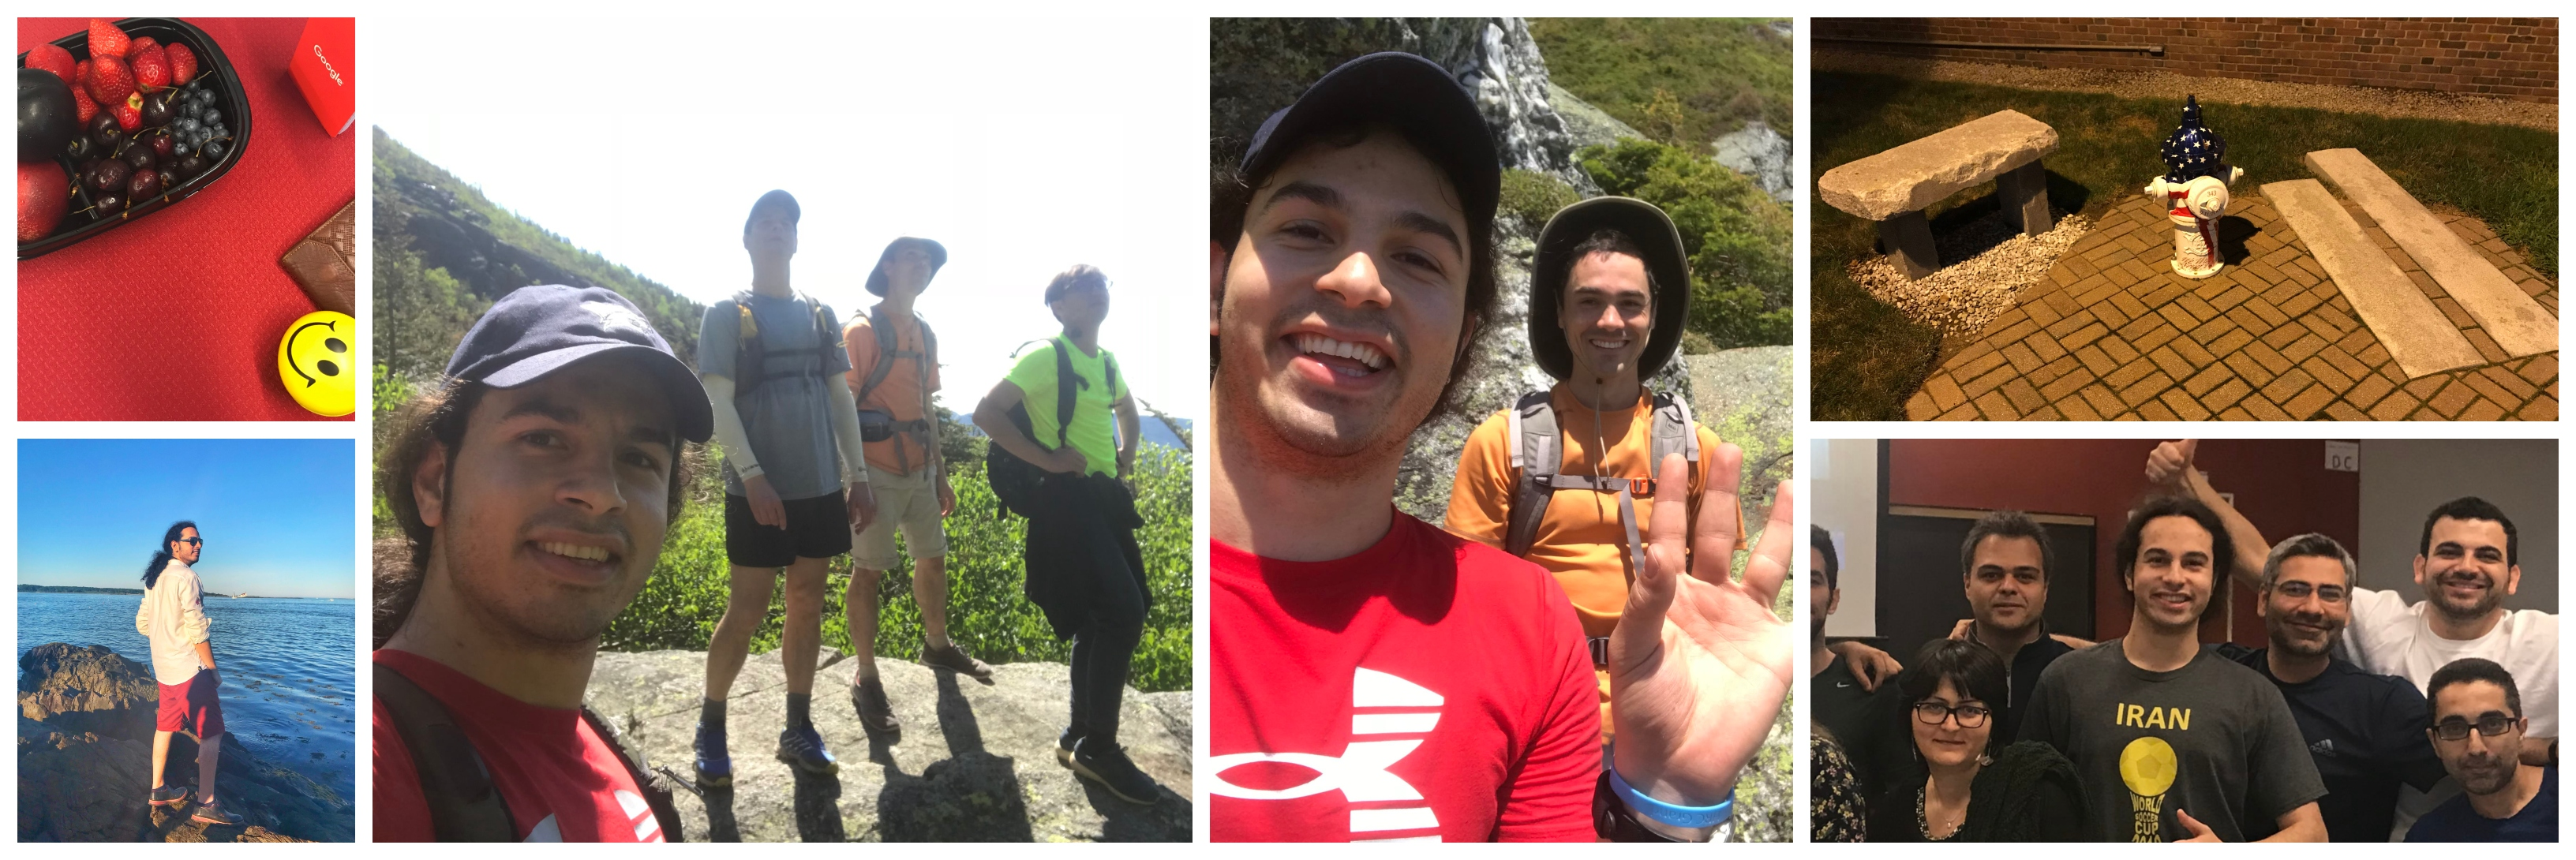
\includegraphics[scale=0.45]{img.jpg}


\end{document}